\section{Acerca del Autor}

\begin{figure}[h]
\begin{minipage}{11.5cm}

\subsection{Reseña}

Leo Soto es egresado de Ingeniería Informática de la USACH, socio de Continuum y
desarrollador para Hashrocket Chile. Como parte de su experiencia en el mundo
OSS, es parte del del equipo de desarrollo de Jython desde el 2008, tras haber
participado en el Google Summer of Code de ese mismo año. También es colaborador
en Mongoid, un ODM para el lenguaje Ruby y MongoDB, una base de datos no
relacional.

Ha dictado charlas fuera del país en la DjangoCon 2008 realizada en el
GooglePlex en Mountain View, y en la PyCon 2009 en Chicago. En el medio nacional
ha participado como expositor en las FLISOL 2009 y 2010, Encuentro Linux 2008 y
2009 y en las Jornadas Regionales del Software Libre 2009.

\end{minipage}
\begin{minipage}{1.7in}
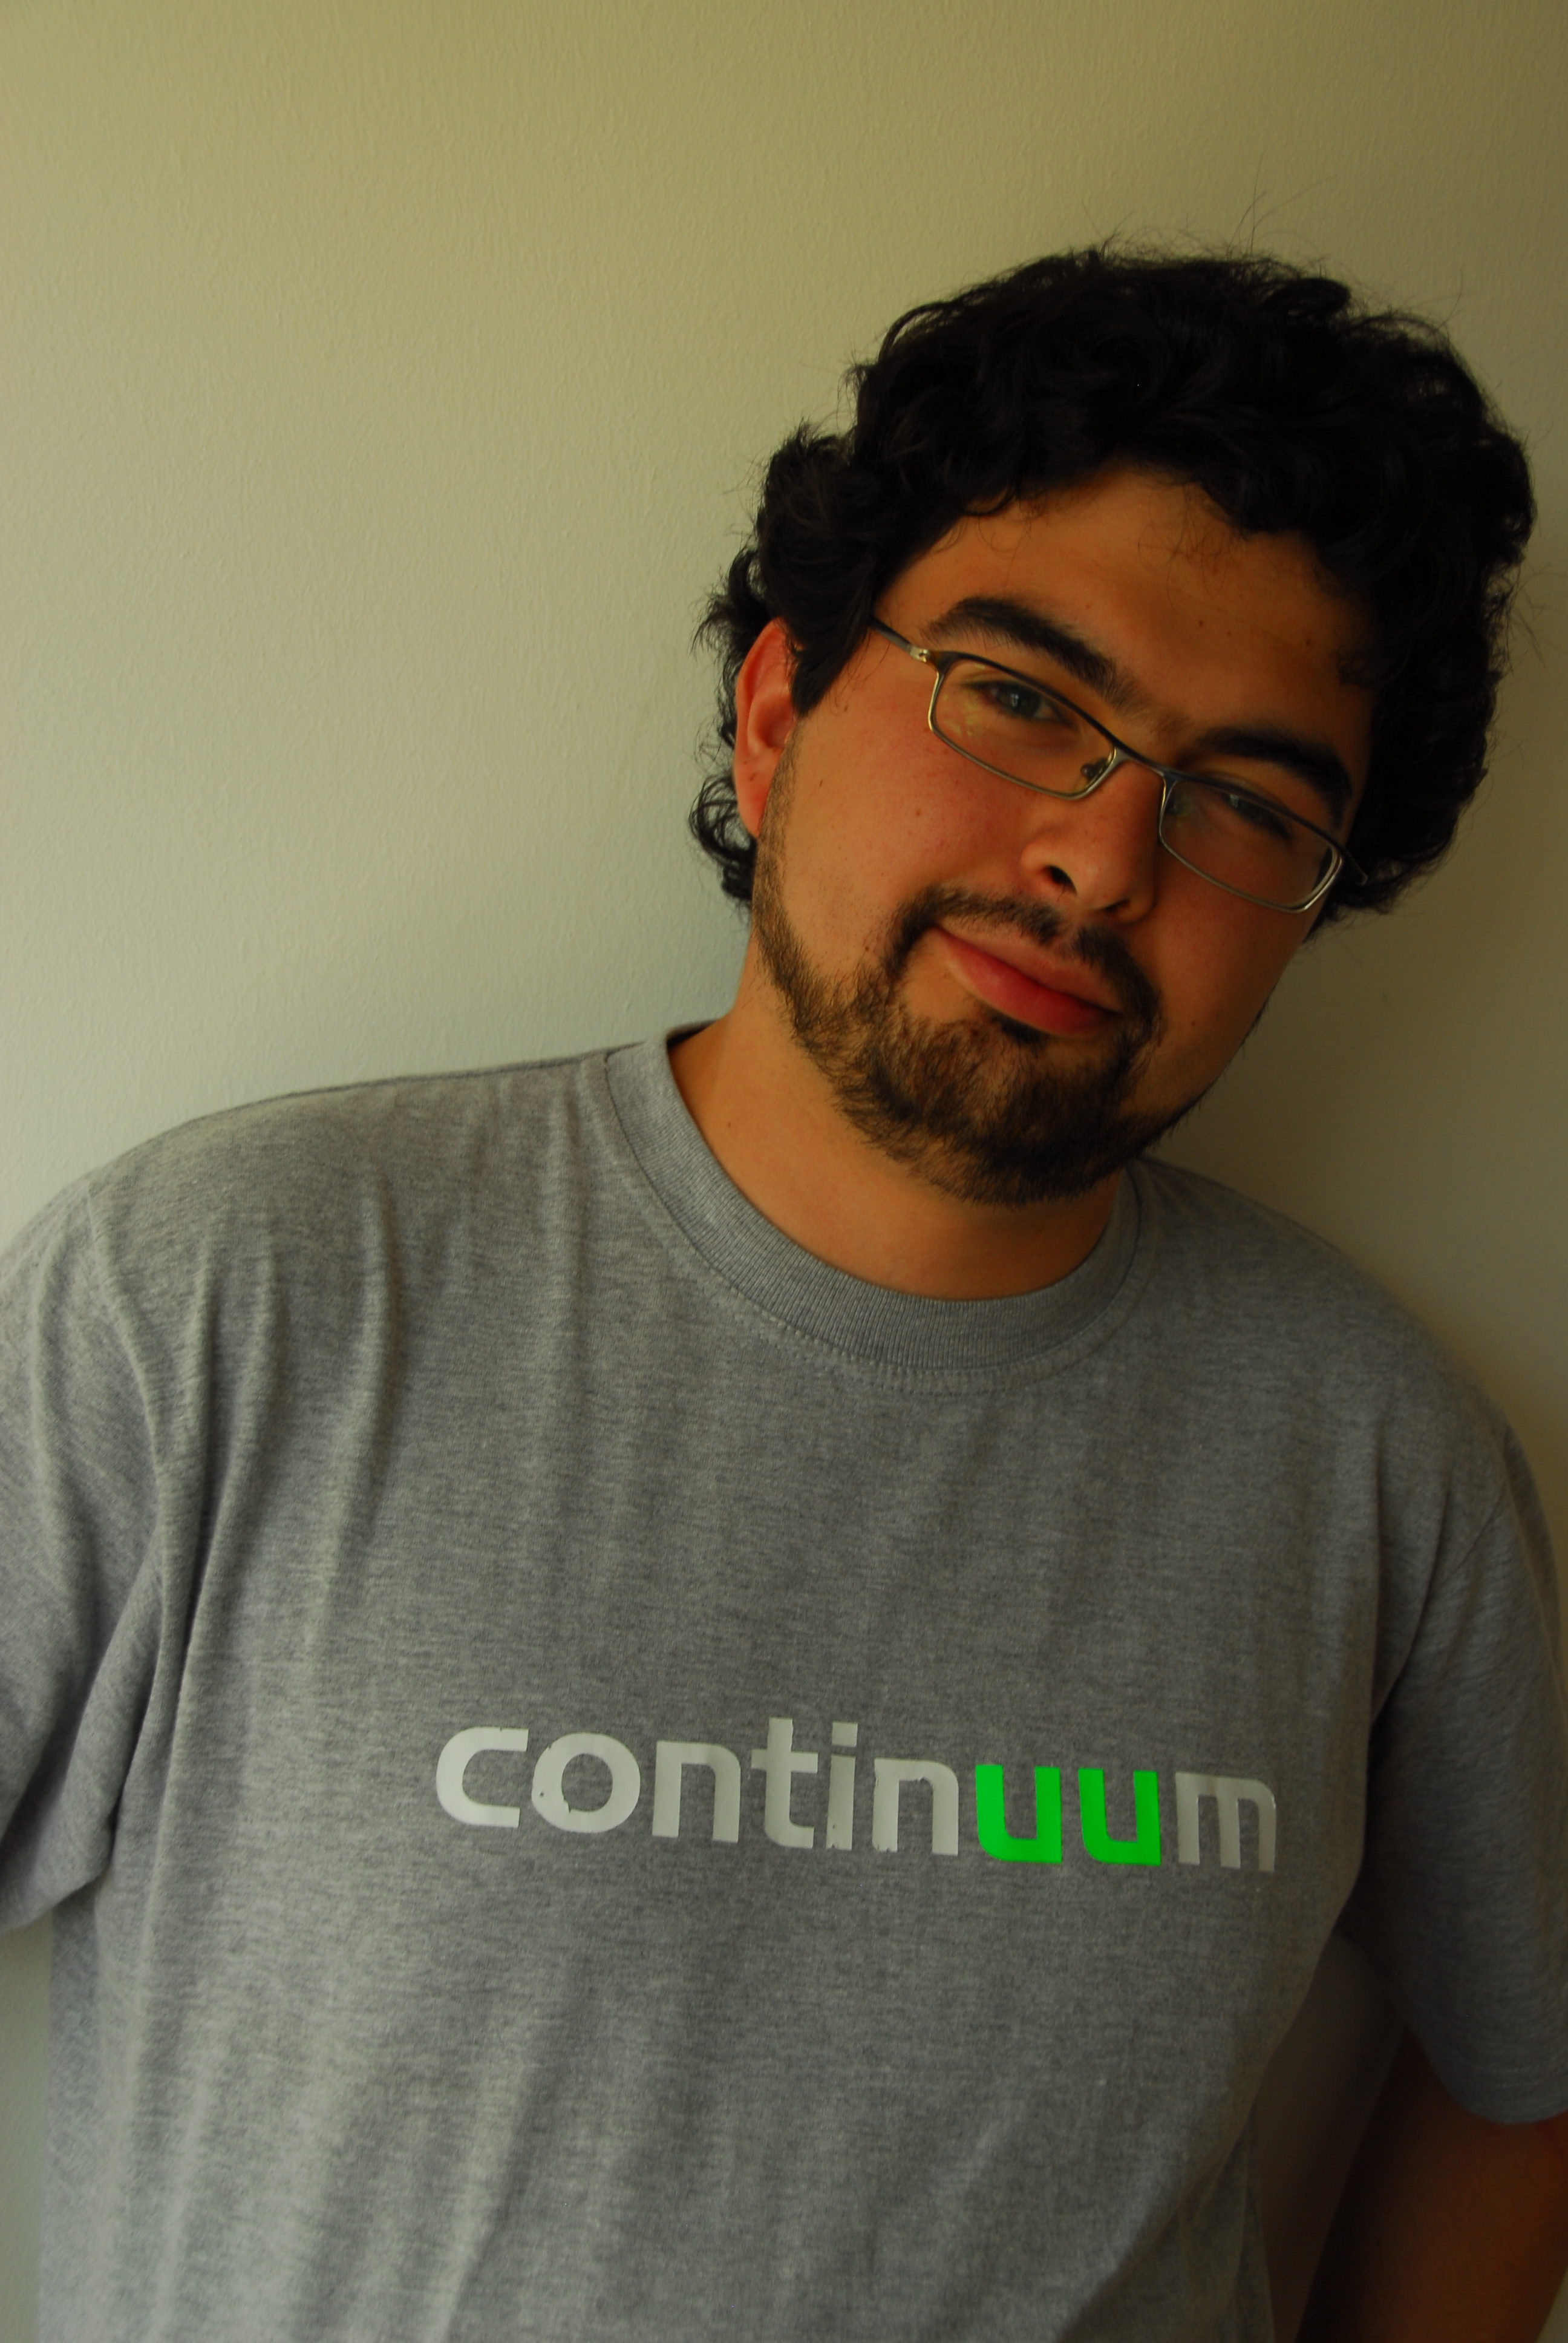
\includegraphics[width=1.5in]{images/DSC_0450.JPG}
\end{minipage}
\end{figure}

\subsection{Datos de contacto}

\begin{itemize}
\item{\textbf{E-mail:} leo.soto@gmail.com}
\item\textbf{{Teléfono:} 9 8733 9008}
\item{\textbf{URL:} \url{http://blog.leosoto.com}}
\end{itemize}
